% intro
% outline

The goal of this thesis is to obtain real-time performance for 3D ultrasound reconstruction. Here, we present the measured performance of the methods described in the two previous chapters, and also identify how much of the computation time is spent on the different algorithmic steps on the device. We will first start by describing the test setup used in the measurements, then we present and discuss the performance obtained on different types of computing hardware (CPU and GPU). Last, the distribution of computation time between the different steps of the reconstruction procedure as well as the amount of memory required is presented and discussed.

% Test setup (hardware and input)
\subsection{Test Setup}

	Table \ref{table:test_computer} shows the hardware specifications of the computer used to measure the results in this chapter, with the different GPUs being used one at the time. All hardware is commercially available as commodity products.
	
	\begin{table}[h]
	\centering
	\begin{tabular}{| l l |}
		\hline
		$\bb{GPU}_1$ & Nvidia Tesla C2050 \\
		$\bb{GPU}_2$ & AMD ATI Radeon HD5870 \\
		$\bb{GPU}_3$ & Nvidia Quadro FX5800 \\
		\textbf{CPU} & Intel Core 2 Quad Q9550 \\
		\textbf{Memory} & 4 x 2 GB DDR3 \\
		\textbf{OS} & Microsoft Windows XP 64 bit \\
		\textbf{Compiler} & Microsoft Visual Studio 9.0 \\
		\hline
	\end{tabular}
	\caption[Test computer specifications]{Test computer specifications. See Table \ref{table:c2050hd5870} for GPU details}
	\label{table:test_computer}
	\end{table}
	
	Table \ref{table:test_input} gives a specification of the test input and volume size that was used for the performance tests. In parentheses are the symbols that from now on will be used to refer to these values. The tracking data were obtained from a Polaris optical tracking system (Northern Digital, Waterloo, Canada), and the b-scans from a Vivid 7 ultrasound scanner (GE Vingmed Ultrasound, Horten, Norway), equipped with a GE M12L linear array probe (GE Healthcare, Waukesha, WI).
	
	\begin{table}[h]
	\centering
	\begin{tabular}{| l l |}
		\hline
		\textbf{Number of b-scans ($n$)} & 434 \\
		\textbf{Number of tracking data} & 520 \\
		\textbf{B-scan size ($w \times h$)} & 768 x 576 pixels \\
		\textbf{Region-of-interest size ($m$)} & 342 x 356 pixels \\
		\textbf{Volume size ($w_{volume} \times h_{volume} \times n_{volume}$)} & 512 x 256 x 512 voxels \\
		\textbf{Pixel spacing x-dimension ($\Delta x$)} & 0.107724 mm \\
		\textbf{Pixel spacing y-dimension} ($\Delta y$) & 0.111732 mm \\
		\textbf{Voxel spacing all dimensions ($\Delta v$)} & 0.08 mm \\
		\textbf{Bits per pixel/voxel} & 8 \\
		\hline
	\end{tabular}
	\caption{Test input data}
	\label{table:test_input}
	\end{table}
	
	Most reconstruction algorithms have one or more parameters that increase the reconstruction quality at the cost of increased computational complexity. In Table \ref{table:test_parameters} a list of important parameter settings is provided for the algorithms that were considered.
	
	\begin{table}[h]
	\centering
	\begin{tabular}{| l l |}
		\hline
		\textbf{PNN} & $5^3$ neighbor voxels used for hole filling \\
		\textbf{VNN} & $5\Delta v$ distance cutoff to b-scans \\
		\textbf{Incremental PNN} & no hole filling \\
		\textbf{Incremental} $\bb{DWOP}_4$ & 4 b-scans interpolated per voxel \\
		\textbf{Incremental} $\bb{DWOP}_8$ & 8 b-scans interpolated per voxel \\
		\textbf{Incremental PT} & cubic interpolation of 4 b-scans per voxel \\
		\textbf{Ray casting} & 800 x 600 pixels (i.e. rays) \\
		\hline
	\end{tabular}
	\caption{Test algorithm parameters}
	\label{table:test_parameters}
	\end{table}

% present performance and speedup, and discuss speedup of GPU vs CPU for various algorithms (incl ray casting)
\subsection{GPU Performance}

	\begin{figure}[h]
	\centering
	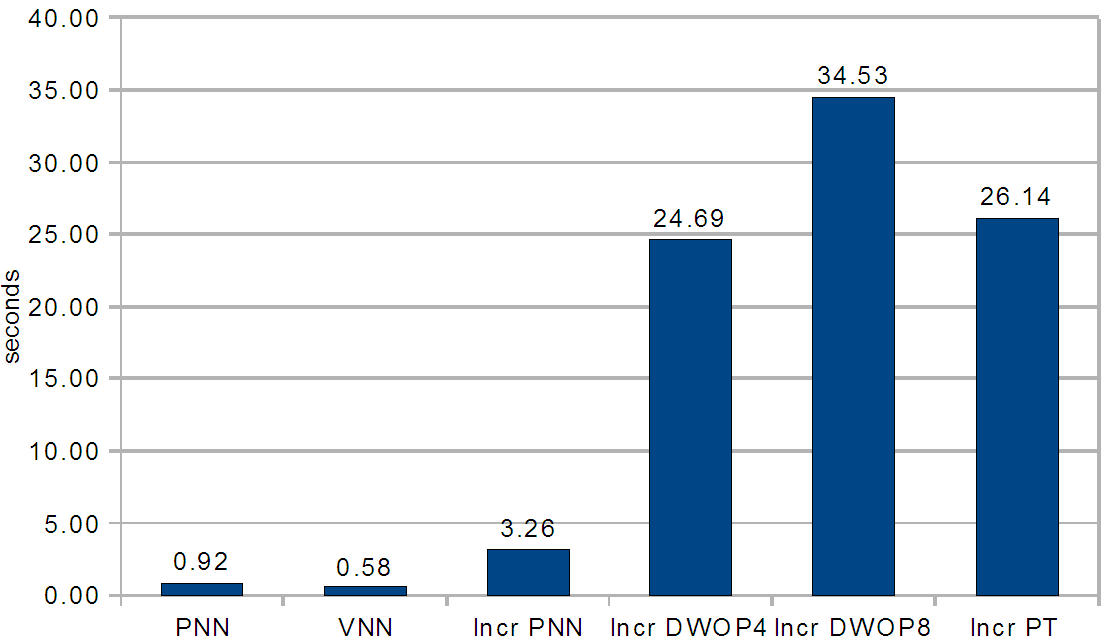
\includegraphics[width=\textwidth]{charts/gpu_performance.png}
	\caption{Reconstruction times using Nvidia Tesla C2050}
	\label{fig:gpu_performance}
	\end{figure}
	
	Figure \ref{fig:gpu_performance} shows the time measured when reconstructing the test input using the Nvidia Tesla C2050 for various algorithms. PNN and VNN are the non-incremental methods, and as one can see, they complete in under one second. The incremental PNN is slower, even without the hole filling, with the reason for this being the overhead associated with incremental reconstruction as previously described. The other incremental methods are substantially slower, and this is due to increased computations resulting in much higher reconstruction quality than the simple PNN. The incremental performance is, however, \emph{real-time} as about 20-30 seconds are typically used for freehand scanning.
	%Note how the incremental reconstruction method in this thesis is substantially better than simply performing a full PNN or VNN for each incoming b-scan. In that case, the reconstruction time would be roughly $434 \times 0.92 = 400$ and $434 \times 0.58 = 252$ seconds, respectively.
	
	The volume size is purposely set at the upper end of what one requires for normal use. Typically, the voxel spacing is set to the same value as the pixel spacing, so given a pixel spacing at around 0.1 mm the volume size would be $450 \times 200 \times 450$ voxels, which is 40 \% less than the one used for testing. The point to note is that these test sizes are \emph{worst case}.
	
	There are two variants of the distance weighted orthogonal projections (DWOP) method examined, which take into account 4 and 8 of the closest b-scans respectively. As can be seen, the increased quality obtained increases the reconstruction time by approximately 40 \%. The $DWOP_4$ and the method based on the probe trajectory (PT) take roughly the same time which can be explained by the fact that they both take 4 b-scans into account for each voxel evaluation. The PT method, however, is somewhat slower, which is explained by the higher degree of interpolation used. The complexity of the PT method is reflected by more complex code, which results in generally higher register use compared to the DWOP (49 \textit{vs.}\ 33 registers).
	
	\begin{figure}[h]
	\centering
	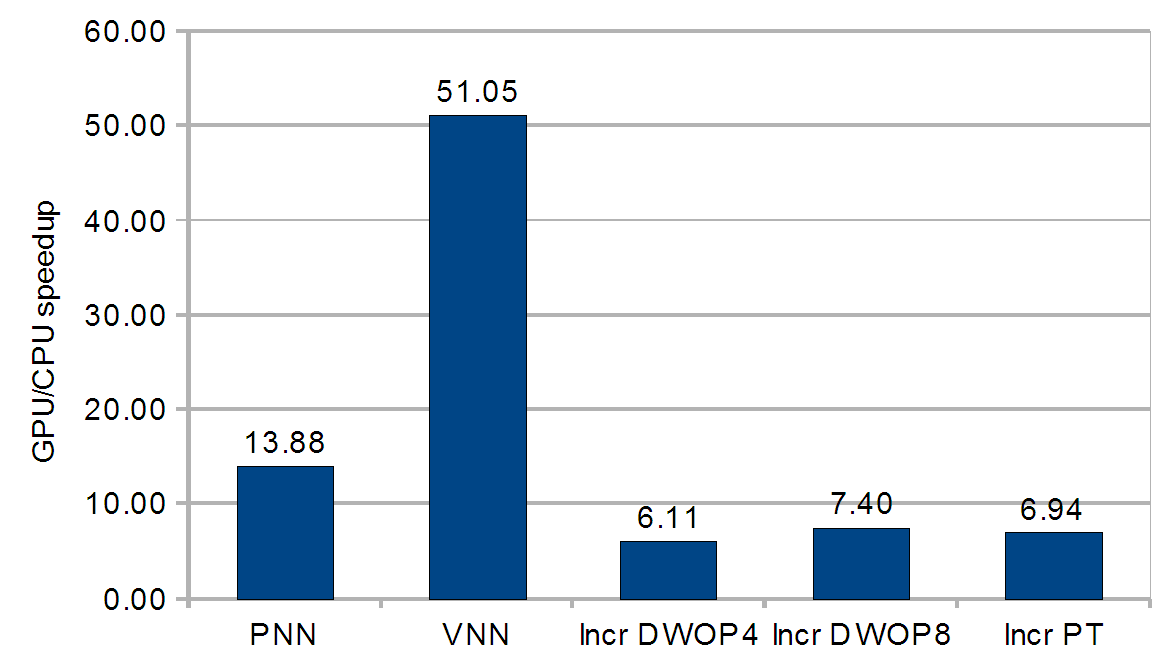
\includegraphics[width=\textwidth]{charts/gpu_cpu_speedup.png}
	\caption{Speedup of Intel Q9550 vs Nvidia Tesla C2050}
	\label{fig:gpu_cpu_speedup}
	\end{figure}
	
	The reconstruction methods were also implemented using only a single-threaded sequential CPU for the computations. In all cases the CPU was slower than the GPU version. Figure \ref{fig:gpu_cpu_speedup} shows the speedup of utilizing the GPU compared to only the CPU, with the performance of the GPU versions between 6 and 14 times faster, and 51 times faster in the case of VNN. In all cases, this is a substantial speedup. The main limiting factor in the speedup of the incremental cases is in the transfer of the volume at each increment (the specifics will be discussed in Section \ref{section:time_distribution}). One can see that the speedups of DWOP and PT are in the same order as their respective computation times. The explanation behind this is that increased computational load means that the processing power of the GPU can be utilized even more, and that the host-device transfers are smaller in comparison to the computations.
	
	While the non-incremental PNN gains a 14 times speedup, the non-incremental VNN gains a significant 51 times increase in performance. Note that these two algorithms are inherently different, and that they therefore cannot be expected to behave similarly to each other when utilizing the massively parallel GPU. One reason is the determinism of the implementations. Each of the threads in VNN reconstruction does exactly the same work, with a small difference at the end of the computations (based on  the voxel being in the ROI or not). For PNN this difference occurs early, as the pixels are processed in the beginning. Such branching results in low occupancy on the GPU, and makes it difficult to achieve good performance. As explained in Section \ref{section:non-incremental_pnn}, one of the major steps of the PNN algorithm is partitioned among "only" 434 threads, one per b-scan. While the VNN can use $w_{volume} \times h_{volume} \times n_{volume} = 512 \times 256 \times 512$ threads, i.e. one per voxel, which is a scalability more suitable to the massively parallel GPU. Furthermore, the hole-filling needed in PNN is a task similar in complexity to the VNN, and thus PNN in total should be slower than VNN. For more details on the difference between VNN and PNN performance, see Section \ref{section:time_distribution}.
	
	%\begin{table}[h]
	%\centering
	%\begin{tabular}{| l l |}
	%	\hline
	%	\textbf{Time for 100 renders} & \textbf{Renders/second (fps)} \\
	%	\hline
	%	\hline
	%	2.81 seconds & 35.6 \\
	%	\hline
	%\end{tabular}
	%\caption{Ray casting performance using Nvidia Tesla C2050}
	%\label{table:raycasting_performance}
	%\end{table}
	
	When using the Nvidia Tesla C2050, \textbf{100 renders} of the $512 \times 256 \times 512$ volume were ray casted in \textbf{2.81 seconds}, which is equivalent to \textbf{35.6 frames per second}. There are many definitions of how many frames per seconds are required to be considered \emph{real-time}, but a lower limit of 25 (PAL television format) or 30 (NTSC television format) should be sufficient. Given a lower limit of 1 update per reconstruction increment, 434 b-scans over 20 seconds would require a frame rate of 21.7. Thus, the performance is more than sufficient for real-time display.

% explain speedup of Fermi vs Quadro and Radeon (and Mac?) for various algorithms
\subsection{Performance of GPU Platforms}

	\begin{figure}[h]
	\centering
	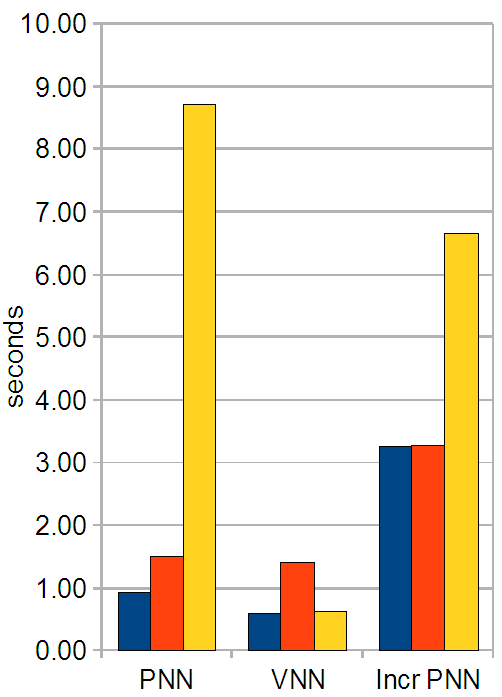
\includegraphics[height=0.33\textheight]{charts/platforms_performance_1.png}
	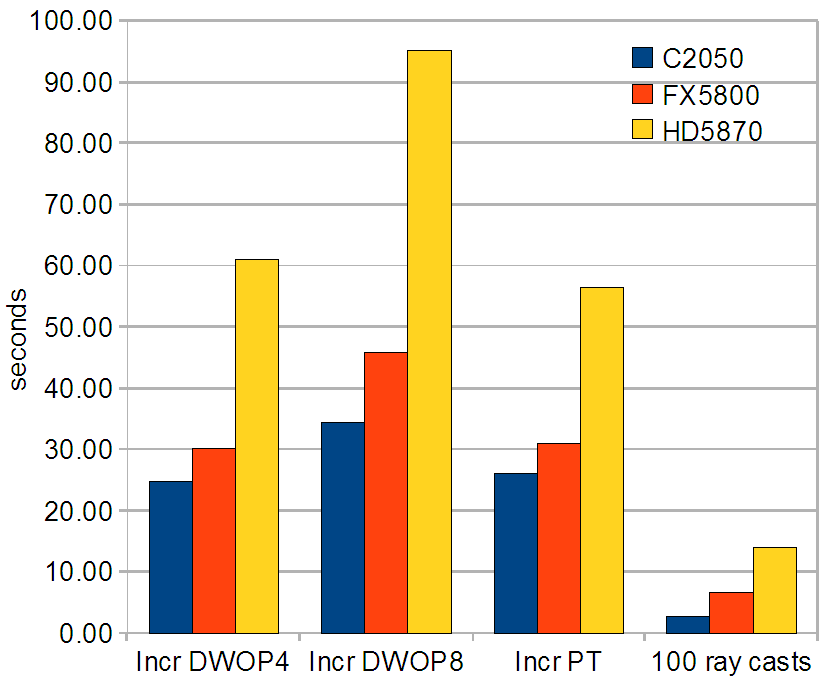
\includegraphics[height=0.33\textheight]{charts/platforms_performance_2.png}
	\caption[Performance of reconstruction and ray casting]{Performance of reconstruction and ray casting on Nvidia Tesla C2050, AMD HD5870 and Nvidia Quadro FX5800}
	\label{fig:platforms_performance}
	\end{figure}
	
	It should now be established that reconstruction performance is substantially greater using the GPU. However, several GPU platforms are available for comparison. The C2050 is at the time of writing the latest and most powerful generation on the market. By using the multiplatform OpenCL standard \cite{openclspec}, it is possible to execute the code on both Nvidia and AMD GPUs. Figure \ref{fig:platforms_performance} shows the performance obtained on the C2050, the older FX5800 also from Nvidia, and the HD5870 from AMD. In terms of prior expectations, the FX5800 is one of the most powerful of the \emph{previous} generation of Nvidia GPUs, and the HD5870 is expected to place itself roughly halfway between these two cards.
	
	With these presumptions, the performance results both confirm and surprise. The C2050 performs better than the FX5800 in all cases, with up to 2.5 times the performance. While in some cases (like incremental PNN) the performance is almost equal or only slightly better, but this will be explained below. The HD5870 however, disappoints in all except in the one case of VNN, with performance typically around 50 \% of the FX5800 and as low as 17 \% in the case of PNN. Just as VNN proved to be very suitable for the GPU with a speedup of 51, it also seems to be the case on the HD5870 and compares favorably with a performance close to the much newer C2050. In the other cases, it can be pointed out that the OpenCL standard was made with CUDA in mind because of its status as a \emph{de facto} standard at the time. AMD's OpenCL implementation obviously has room for improvement, and the potential is clearly there as seen with the performance of VNN. It should be noted however, that in all the cases the HD5870 is still between 1.5 and 3.2 times faster than the pure CPU implementation (and 47 times faster for VNN).
	
	As mentioned, the C2050 beats the older FX5800 in all the cases, but one notices that the gap is substantially narrower for the incremental methods. The explanation in these cases is due to the time spent on transferring the volume. Even though C2050 represents the next generation of Nvidia GPUs, the data bus between host and device (PCI Express) is identical for both. This is evident in the cases of incremental reconstruction, where the computations are lighter for each increment. Again, this is confirmed by a greater relative gap (1.23 \textit{vs.}\ 1.33) between $DWOP_4$ and $DWOP_8$, where the only difference is computational complexity.
	
	In the case of VNN and ray casting, the C2050 offers 2.5 and 2.4 times the performance of the FX5800, but the C2050 has only about twice the number of computational cores of the FX5800 and 40 \% increased memory bandwidth \cite{c2050, fx5800}. The explanation is one key feature to the Fermi GPU architecture which C2050 belongs to, the addition of L1 and L2 cache. With a L1 cache per streaming multiprocessor and a global L2 cache for all computation cores, the effective memory bandwidth can be drastically increased depending on the application. If the same data is read repeatedly by several threads, the values will be available in this fast cache. This is especially the case for VNN, where the b-scan plane equations and corner points are read repeatedly by neighboring threads, and also for ray casting where neighboring rays read the same voxel data. In both cases it is hard to estimate exactly which groups of threads will require what groups of common data, but the cache handles this temporal locality automatically.

% which steps of algorithms take how long computation time w/ explanation
	% steps on GPU (i.e kernels)
	% CPU steps (interpolation, calibration, setting up data structures, etc)
\subsection{Distribution of Reconstruction Time}
	\label{section:time_distribution}
	
	To gain a deeper understanding of the reconstruction performance for each method, one has to look at the time is takes to do the various reconstruction steps and the data transfers between device and host. In this section we present this distribution, and explain why it occurs like it does. In all cases, the C2050 has been used for the measurements. 
	
	\begin{figure}[h]
	\centering
	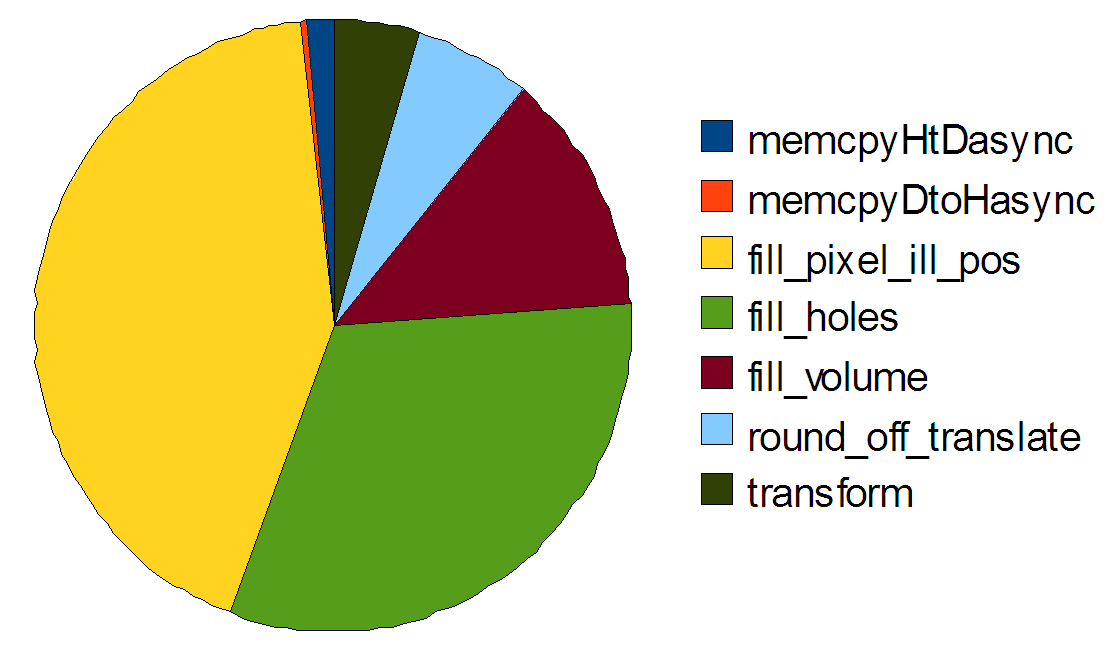
\includegraphics[height=0.3\textheight]{charts/pnn.png}
	\caption[Distribution of computation time for PNN]{Distribution of computation time on Nvidia Tesla C2050 for PNN}
	\label{fig:pnn_pie}
	\end{figure}
	
	Figure \ref{fig:pnn_pie} shows the distribution of the time for PNN on the GPU. Note that transfers between host and device (memcpyHtoDasync and memcpyDtoHasync) are negligible compared to the computations. In this case, around 200 MB (mainly from b-scans) is transferred to the device and 67 MB (the volume) is transferred back. The GPU is connected to the host via a PCI Express 2.x 16X bus, which has an upper transfer limit of 8 GB/s. These small data sizes are thus negligible. The largest portion is the task of filling $pixelill$ and $pixelpos$, and as previously discussed, this is hard to parallelize, and is indicated by a GPU core occupancy of only 17 \% during this step. The rest of the steps all have a 100 \% occupancy. However, there are two other tasks that also take up a large part of the time: filling the volume and (especially) filling the holes. Actually, processing all the ROI-pixels and inserting them into the volume actually takes less time than filling those holes. This demonstrates how the PNN performance is penalized by the hole filling required due to of the nature of the algorithm.
	
	\begin{figure}[h]
	\centering
	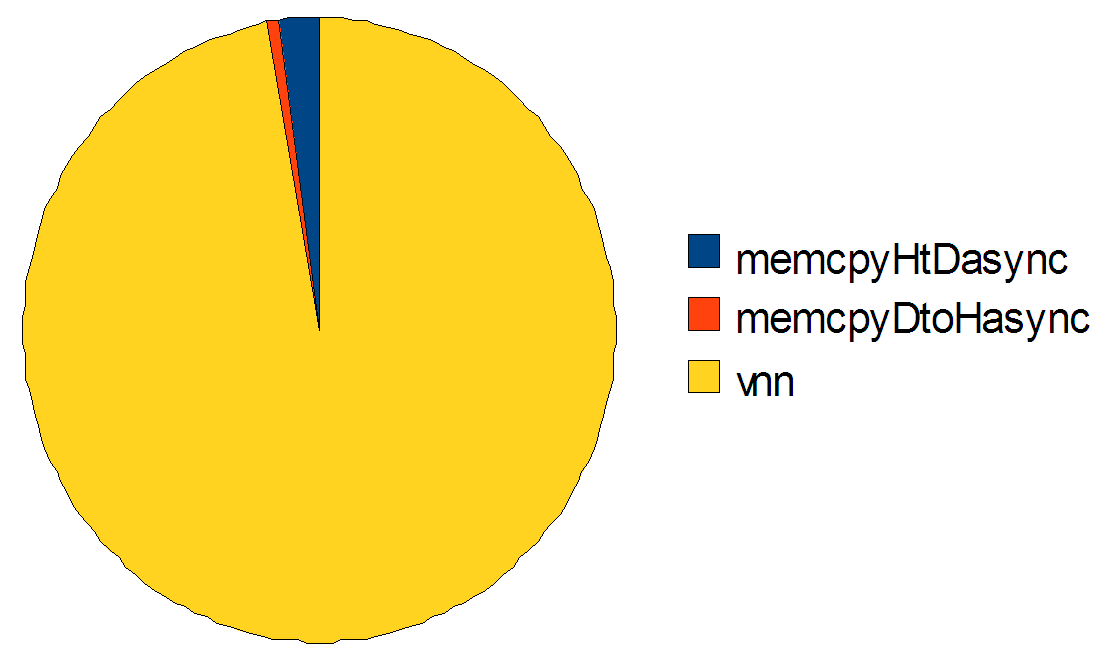
\includegraphics[height=0.3\textheight]{charts/vnn.png}
	\caption[Distribution of computation time for VNN]{Distribution of computation time on Nvidia Tesla C2050 for VNN}
	\label{fig:vnn_pie}
	\end{figure}
	
	Figure \ref{fig:vnn_pie} shows the distribution of time for VNN on the GPU. As in the case with PNN, the transfers between host and device are negligible (in fact, they are of the same absolute sizes as in PNN). Unfortunately, the VNN reconstruction was implemented as a single GPU kernel, and thus the distribution between steps cannot be identified.
	
	\begin{figure}[h]
	\centering
	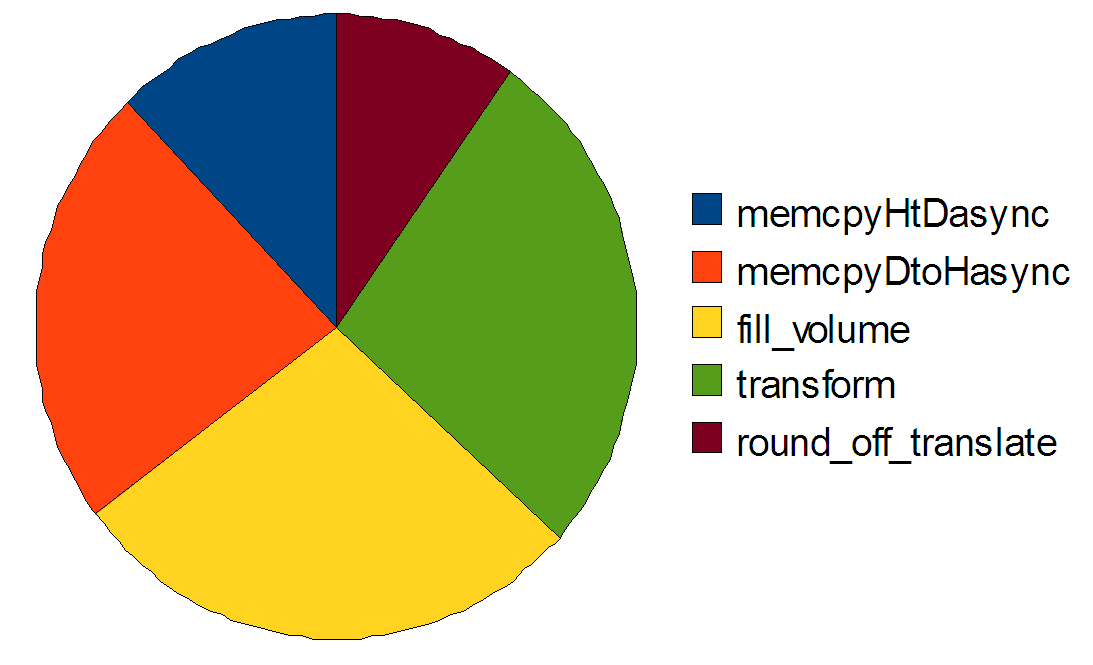
\includegraphics[height=0.3\textheight]{charts/incr_pnn.png}
	\caption[Distribution of computation time for incremental PNN]{Distribution of computation time on Nvidia Tesla C2050 for incremental PNN}
	\label{fig:incr_pnn_pie}
	\end{figure}
	
	Figure \ref{fig:incr_pnn_pie} shows the distribution of time for incremental PNN on the GPU. As opposed to the non-incremental cases, transfers between host and device take a noticeable share as more than a third of the time is now consumed on this. For each increment, a tracking matrix and the $pixelpos$ and $pixelill$ for one b-scan must be transferred, approximately 1.6 MB. The transfer back of the transformed $pixelpos$ is approximately 1.4 MB. However, the overhead associated with each transfer adds up, as demonstrated by the large share of the total time. This overhead is especially noticeable for incremental PNN, due to the total time spent per increment being relatively smaller.
	
	\begin{figure}[h]
	\centering
	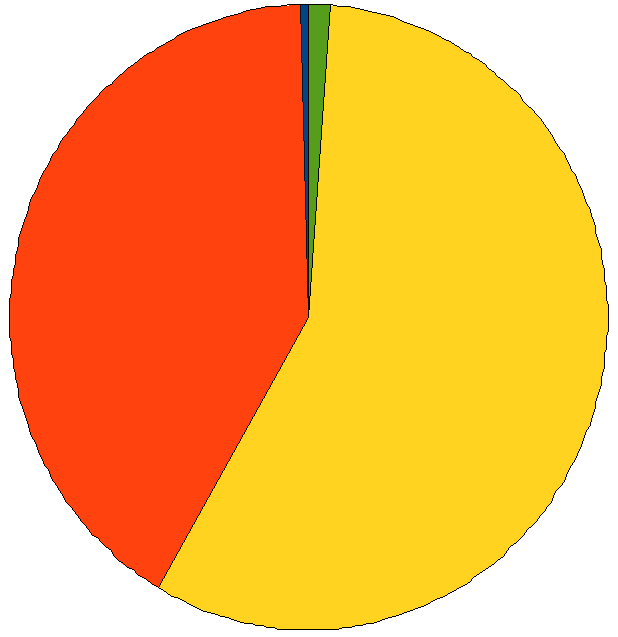
\includegraphics[height=0.175\textheight]{charts/incr_hq_1.png}
	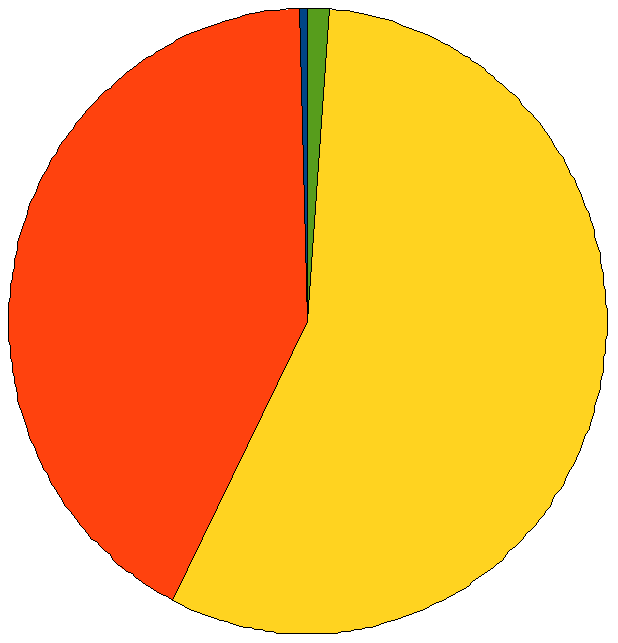
\includegraphics[height=0.175\textheight]{charts/incr_hq_2.png}
	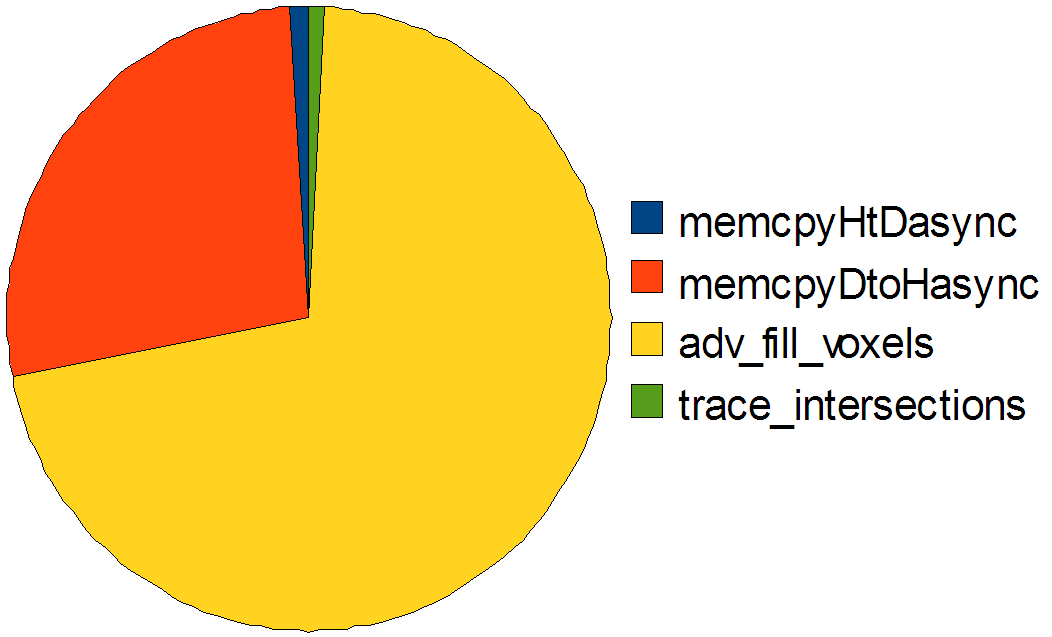
\includegraphics[height=0.175\textheight]{charts/incr_hq_3.png}
	\caption[Distribution of computation time for PT, $DWOP_4$ and $DWOP_8$]{Distribution of computation time on Nvidia Tesla C2050 for PT, $DWOP_4$ and $DWOP_8$}
	\label{fig:incr_hq_pie}
	\end{figure}
	
	The other incremental methods share the same characteristics in the time distribution, as shown in Figure \ref{fig:incr_hq_pie}. The transfers between device and host take up a big share, but this is only \emph{from} the device \emph{to} the host, as host to device is practically negligible. The reason for this is that as each increment takes a substantially longer time in these methods than in incremental PNN, and the overhead of the small host-to-device transfer is hidden, while transferring the 67 MB volume for each increment still takes its share of the total time. The same reasoning explains why $DWOP_8$ has a smaller share of transfers than $DWOP_4$; i.e.\ each increment is more computationally complex. In fact, incremental PT and $DWOP_4$ has almost identical time distributions, which is not surprising as their computational complexity is very similar. As can be seen in the charts, the task of finding the voxels between two b-scans (trace\_intersections) is negligible, rather is the filling of those voxels by PT or DWOP that take up all the computation time.
	
	\begin{figure}[h]
	\centering
	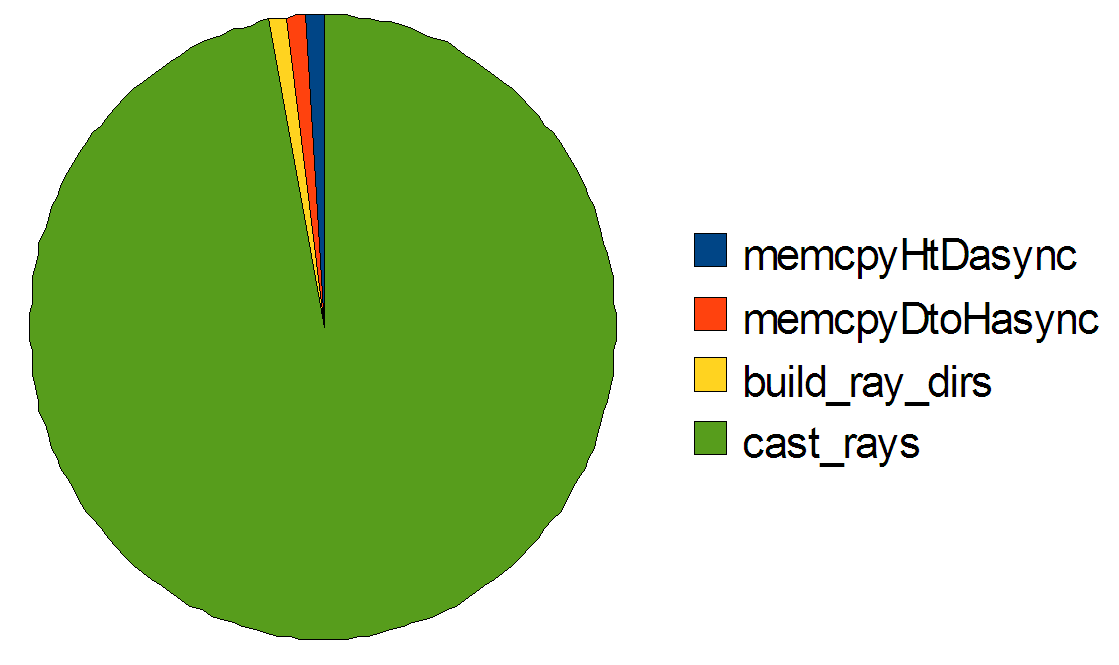
\includegraphics[height=0.3\textheight]{charts/ray_casting.png}
	\caption[Distribution of computation time for ray casting]{Distribution of computation time on Nvidia Tesla C2050 for ray casting}
	\label{fig:ray_casting_pie}
	\end{figure}
	
	Figure \ref{fig:ray_casting_pie} shows the distribution in the time for ray casting on the GPU. One quickly sees that transfers between host and device are negligible, as is expected given only a few camera parameters are sent to the device and a 480 KB rendered frame is sent back. This demonstrates the advantage of already having the reconstructing volume in the device memory, making additional transfers unnecessary. Building the ray directions is also a simple task, as demonstrated in the chart, and this is easily explained when one takes into account that the number of rays to be built is only $800 \times 600 = 480,000$, while the number of voxels to be sampled is $512 \times 256 \times 512 = 67,108,864$.
	
% present and discuss how much memory is used in all algs (make table with buffers and total)
\subsection{Memory Use}

	\begin{figure}[h]
	\centering
	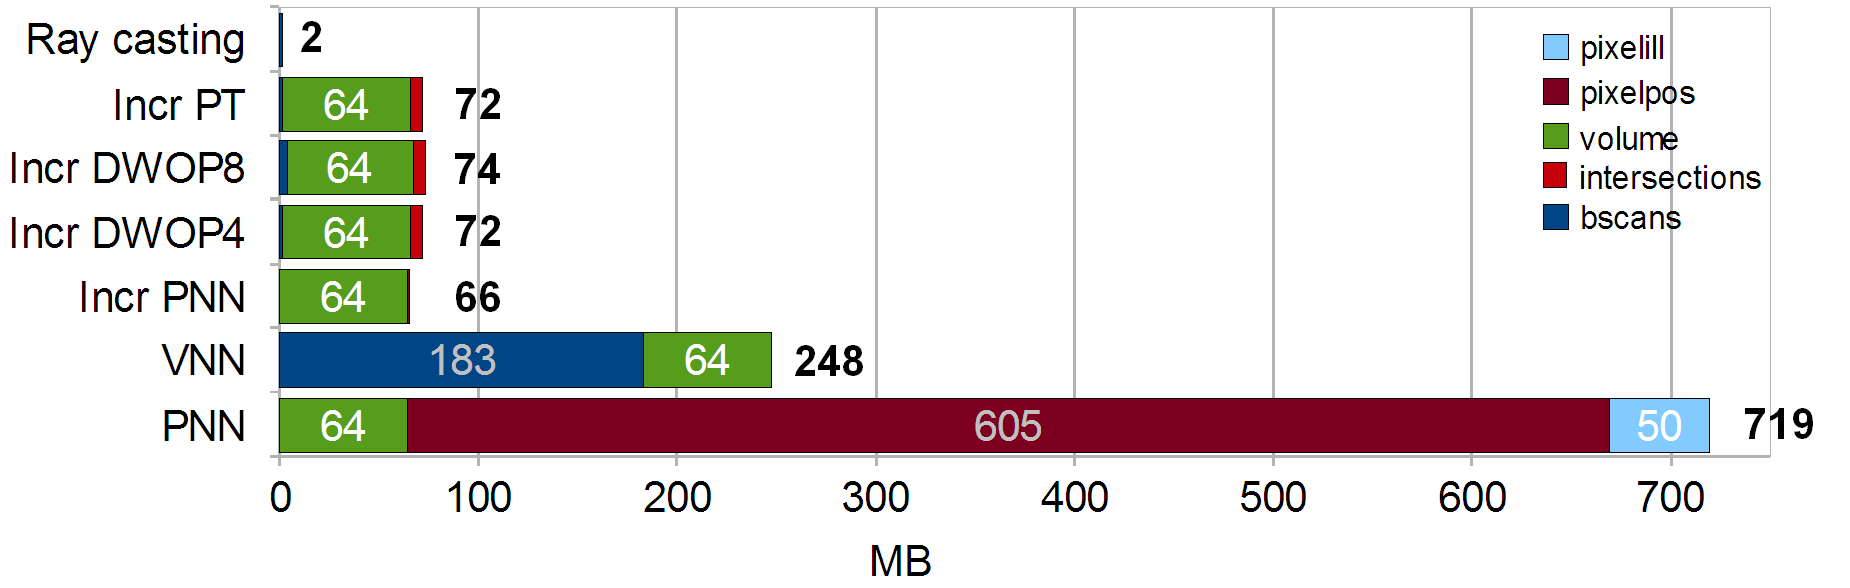
\includegraphics[width=\textwidth]{charts/memory_use.png}
	\caption{GPU memory use}
	\label{fig:memory_use}
	\end{figure}
	
	The chart in Figure \ref{fig:memory_use} shows how much GPU memory is used by each reconstruction method and the ray casting when using the previously described test data as input. It is easy to see that PNN uses the most memory, a total of 719 MB. Actually, it also requires 183 additional megabytes for the input b-scans, but as these are processed into the 50 MB $pixelill$ at the beginning of the procedure they can subsequently be freed from the GPU memory, hence they are not shown in the chart. The biggest contribution to PNN's memory usage is the $pixelpos$, and this is not surprising with three 4-byte coordinates required per pixel. The VNN on the other hand, requires only the input b-scans and output volume. In all cases, there are negligible amounts of memory used for tracking data, timetags, etc. These are so insignificant that they are not noticeable in the chart, and are so not of interest in this discussion.
	
	The incremental methods are quite similar in that they do not use much memory except for the volume, because the input is processed in small chunks at the time. While incremental PNN only keeps a single b-scan in memory at the time, incremental DWOP and PT utilize a "window" of b-scans and other data as previously described in Section \ref{section:incr_hq_impl}. $DWOP_4$ and PT have a window size of 4, resulting in approximately 1.7 MB for b-scans and other data, while $DWOP_8$ uses 8, requiring approximately 3.5 MB, all relatively small amounts of data. The ray casting of course needs a volume to render, but it is assumed that this is already present in the device memory, and so only an additional 2 MB is required (and most of it is the rendered frame).

% present and discuss how the algorithms scale with problem size (and processing capacity?)
	% voxel-based vs.\ pixel-based computational complexity (big-oh-ish)
	% computation complexity of incremental approach (big-oh-ish)
	% ? measure and make some scaling graphs of the most relevant parameters
%\subsection{Scaling}